\begin{figure}[h!]
	\centering
		\captionsetup{font=small, width=0.8\textwidth}
	\caption{The top panel shows the annualised (log)  risk-premia on  real and nominal bonds, $\E\left[r_{n,t+1}^{b}-r^f_{t+1}\right]$, and $\E\left[r_{n,t+1}^{nb}-r^f_{t+1}\right]$, respectively, as a function of its maturity, $N$, in months. The middle panel shows its volatility, whilst the bottom one shows the Sharpe Ratio.}\vspace{0.25cm}
	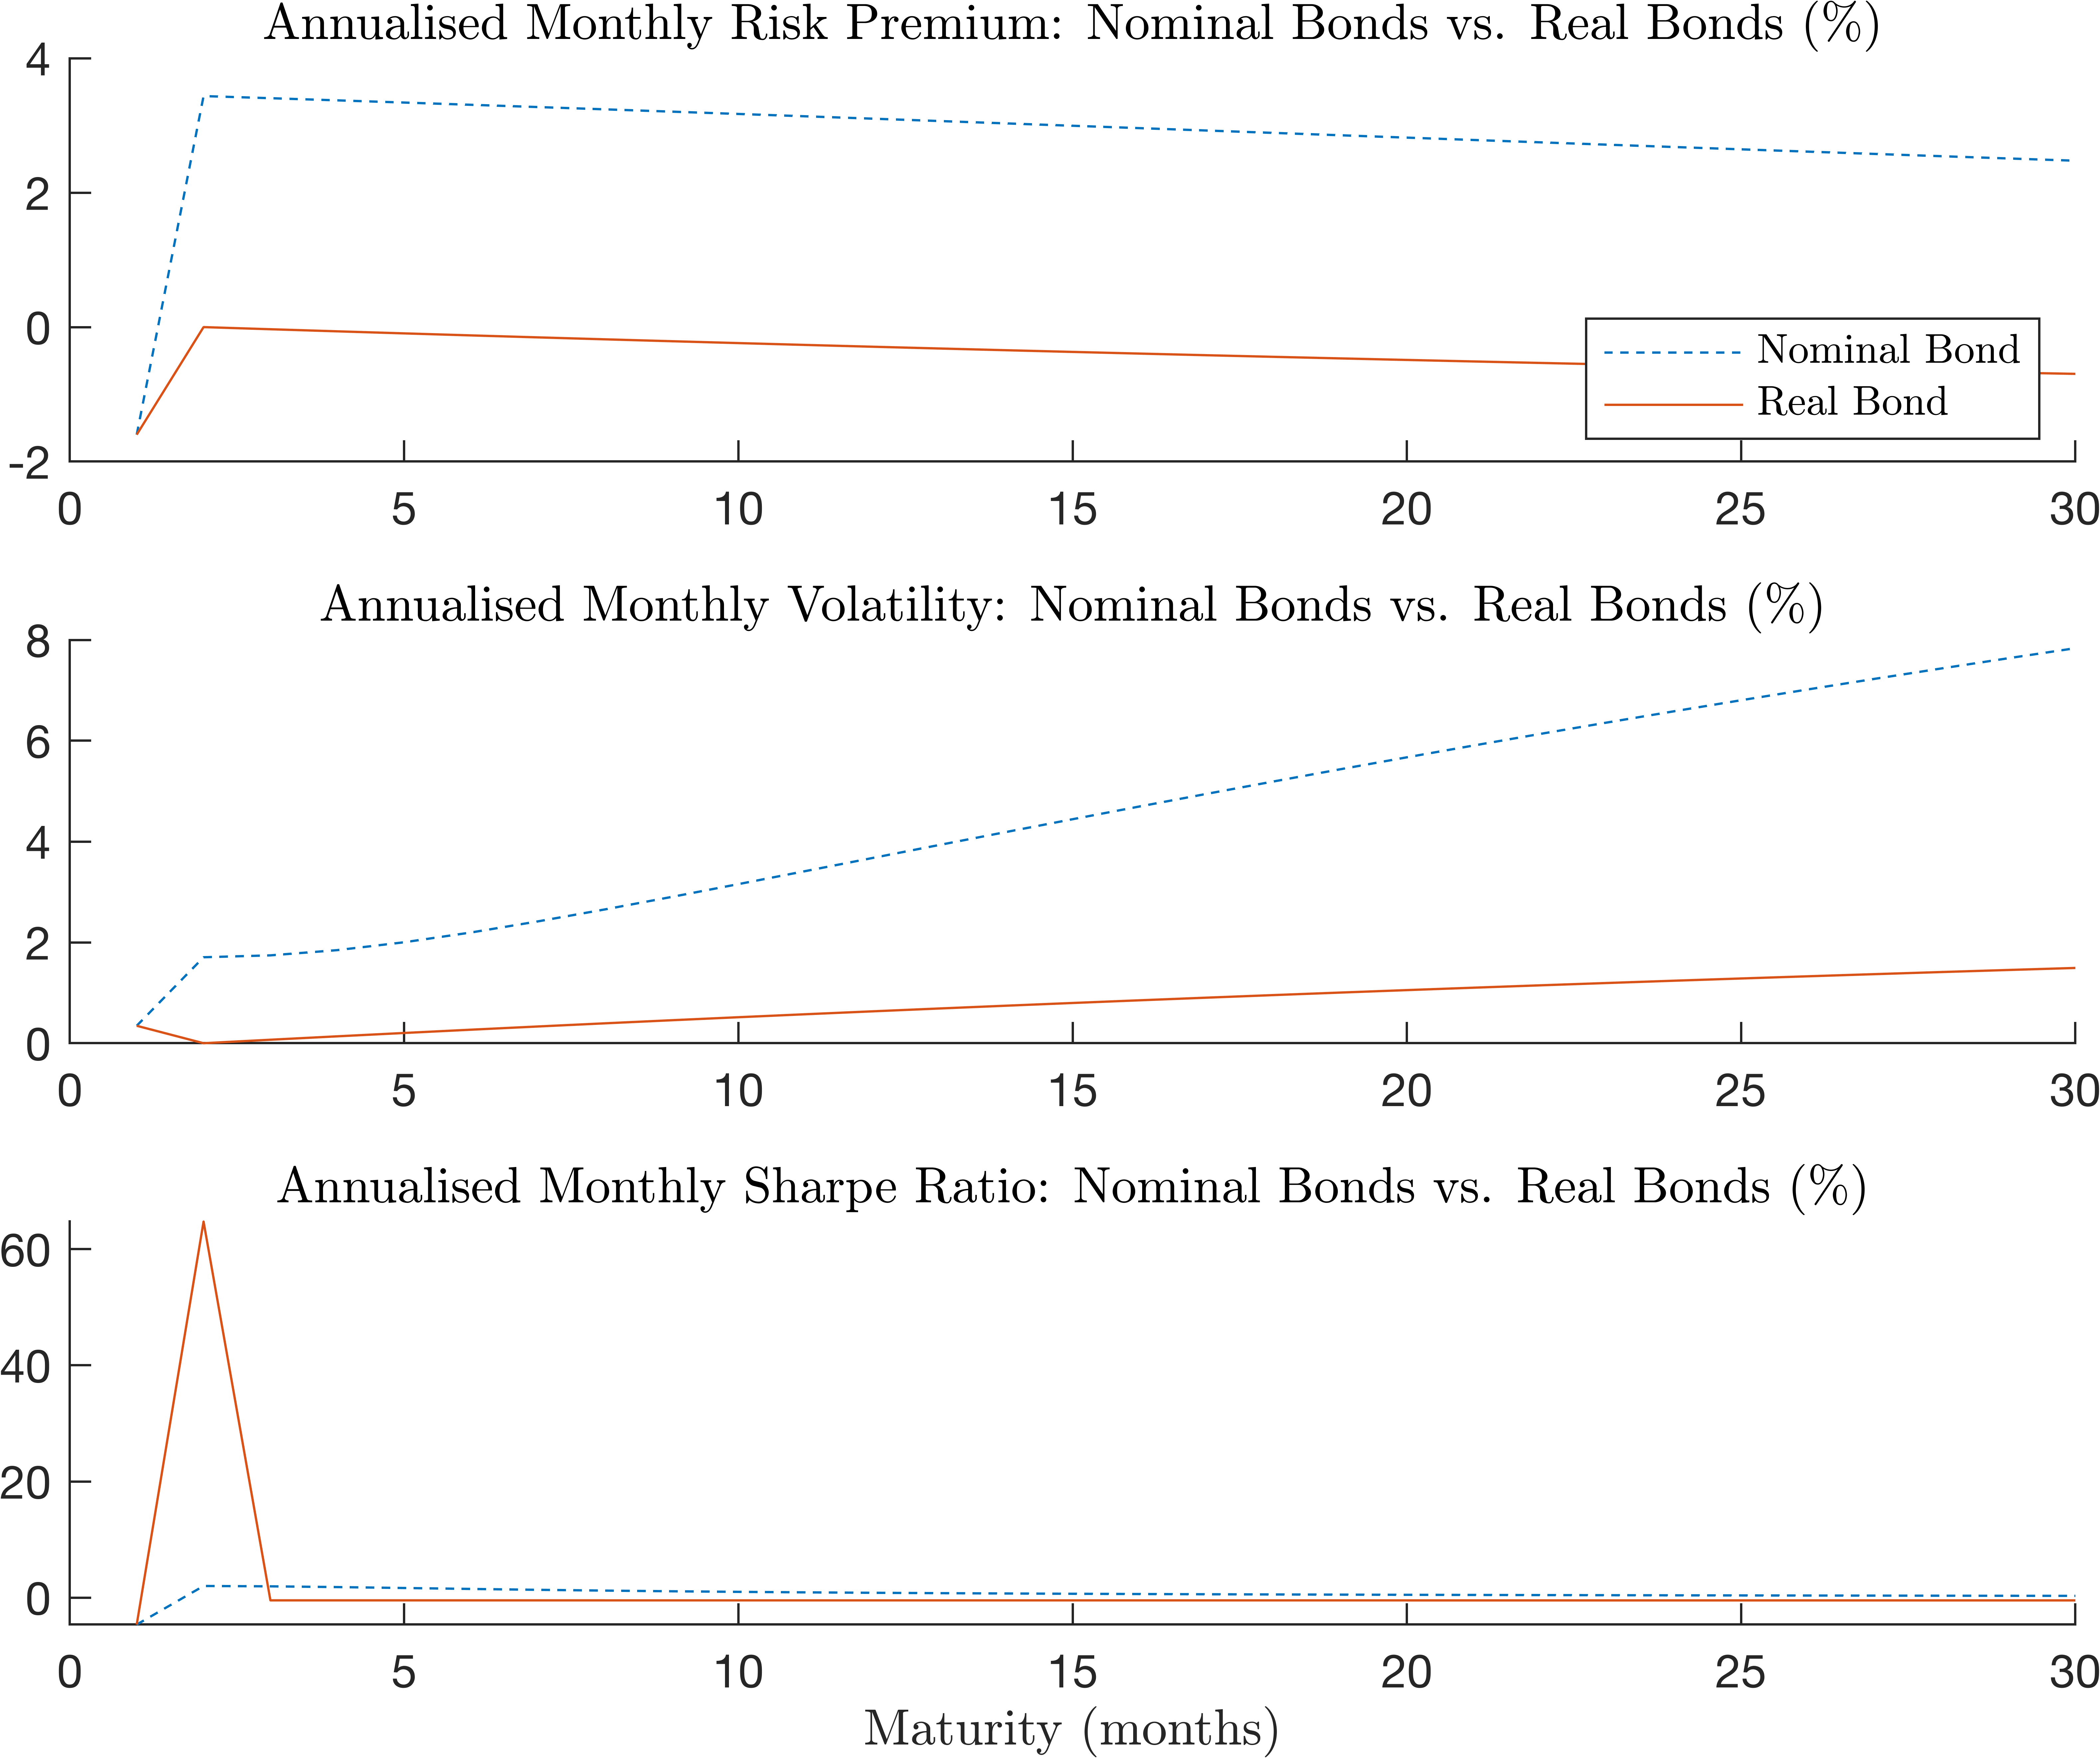
\includegraphics[scale=0.7]{secs/fig/realvsnominal.png}
\end{figure}